\documentclass[a4paper]{article}
\usepackage[utf8]{inputenc}
\usepackage{graphicx}
\usepackage{color}
\newcommand{\unam}{\,\mathrm{u}^2}
\newcommand{\una}{\,u$^2$}
\newcommand{\un}{\,u}
\newcommand{\unm}{\,\mathrm{u}}

\newcommand{\len}{\mathrm{length}}
\usepackage{amsmath}
\usepackage{amssymb}
\usepackage{fullpage}
\usepackage[final]{pdfpages}
\title{COMP2911 Project: Revised Design} 
\author{Stephen Sherratt, Matthew Todd, Rebecca Wiley}
\begin{document}
\maketitle


\section{Changes Since Preliminary Design}

The following changes were made to the design since the preliminary design.


\subsection{Removal of Gap class}

Since being given a recommended way to represent walls (top left square and direction), 
    we changed our design slightly so as to not need a way of representing the gap between squares.
Walls are now represented in this way.
The main reason for representing walls using gaps was to get constant time lookups of which wall is in each gap.
In the revised design, constant time lookups are still possible by representing the collection of walls in a hashset.

\subsection{Renaming}

Piece has been renamed to Pawn. \\
Move has been renamed to GenericMove.

\subsection{Abstraction}

The class names in the preliminary design now correspond to interface names.
The corresponding class names are now appended with "Impl".
For example the class implementing the Wall interface is named WalledImpl.
Every class has a corresponding interface except for Manager (the class with a main method).

\subsection{Addition of Parser interface and ParserImpl class}

There are two cases in the project when it will be necessary to parse input: in the Manager class to load, 
    save and create games, and in the GameImpl class to read moves.
It would be useful to have a standard way of parsing commands (rather than writing a specific parser for each case).
To solve this, a Parser is used.
This is an object that is created with a list of valid commands and tokens.
This object then has methods related to reading input and returning tokens.



\pagebreak

\section{Revised Class Diagram}

\begin{tabular}{p{12cm}}
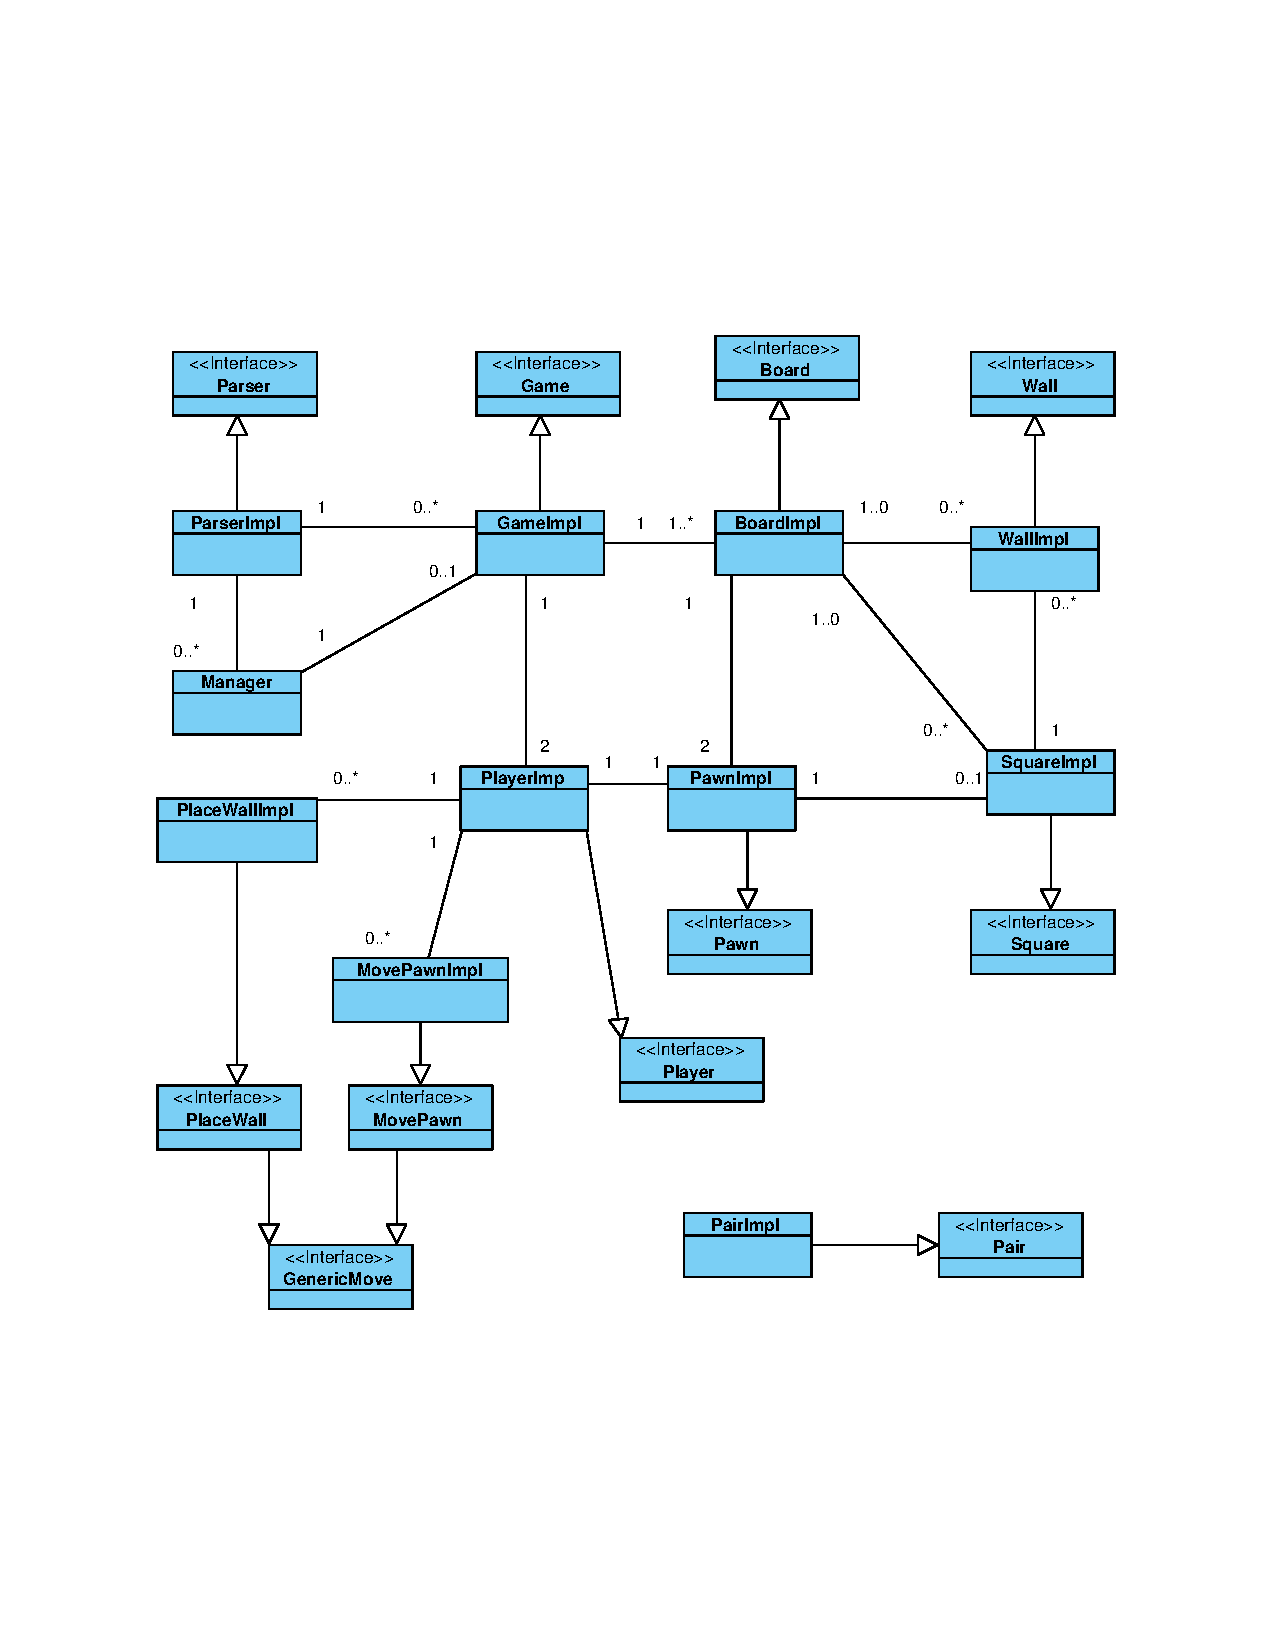
\includepdf[scale=1]{classdiagram.pdf}
\end{tabular}

\vspace{19cm}
\subsection*{Notes}
The diagram does not show the relationships between PairImpl and other classes.
This is because Pair is a utility that is commonly used throughout the project, whenever a pair of items is required.

\end{document}
